\documentclass[aspectratio=169]{beamer}
% \usepackage{enumitem}
\usepackage[utf8]{inputenc}
\usepackage{amsmath, amssymb, amsthm}
\usepackage{algorithm2e}
\usepackage{tikz}
\usepackage{amsmath, amsthm, amssymb}
\usepackage{pgfplots}
\newcommand{\hs}[1]{\hspace*{#1cm}}
\newcommand{\vs}[1]{\vspace*{#1cm}}

\title{Adversarial Uncertainty Quantification in Physics-Informed Neural Networks}
\author{Yibo Yang, Paris Perdikaris}
\institute{University of Pennsylvania}
\date{26.05.2023}

\begin{document}

\maketitle

\section{Introduction}

\begin{frame}{The model: UQPINN}
\begin{minipage}{0.6\textwidth}
{\huge UQPINN = GAN + PINN}
\end{minipage}\hfill
\begin{minipage}{0.4\textwidth}
\begin{enumerate}
    \item \textbf{UQPINN} : Uncertainty Quantification Physics-Informed Neural Network
    \item \textbf{GAN} : Generative Adversarial Network
    \item \textbf{PINN} : Physics-Informed Neural Network
\end{enumerate}
\end{minipage}
\end{frame}

\begin{frame}{Novalty}
"we will develop a flexible \textcolor{orange}{variational inference} framework 
that will allow us to train such models directly from \textcolor{orange}{noisy input/output data}, 
and predict outcomes of non-linear dynamical systems that are partially \textcolor{orange}{observed}
with quantified \textcolor{orange}{uncertainty}"
\hs{1}
\begin{flushright}
    \textit{-- Yibo Yang, Paris Perdikaris}
\end{flushright}
\hs{2}
\begin{center}
\uncover<2->{
    Using adversarial approach to handle randomness in observations.  
}
\end{center}
\end{frame}

\section{Experiment}

\begin{frame}{Experiment Setup}
\begin{tabular}{p{0.2\textwidth}p{0.4\textwidth}p{0.4\textwidth}}
    &{\Large Author's Experiment Setup} & \uncover<2->{\Large My Experiment Setup}\\[0.5cm]

    \textbf{GPU} & NVIDIA Tesla P100(16GB) & \uncover<2->{MX450(2GB)}\\[0.2cm]
    
    \textbf{DL framework} & Tensorflow v1.10 & \uncover<2->{Pytorch v1.9.0}\\[0.2cm]
   
    \textbf{Formula} & \begin{enumerate}
        \item pedagogical ODE
        \item Burgers' equation
        \item Darcy flow
    \end{enumerate} & \uncover<2->{\begin{enumerate}
        \item pedagogical ODE
        \item Burgers' equation
        \item Darcy flow
    \end{enumerate}}\\
    
    \textbf{Model} & UQPINN & \uncover<2->{\begin{enumerate}
        \item UQPINN
        \item PINN
    \end{enumerate}}\\
\end{tabular}

\uncover<3->{    
\centering
    parameters are set to be the same as the author's
}
\end{frame}

\begin{frame}{pedagogical ODE}
% This file was created with tikzplotlib v0.10.1.
    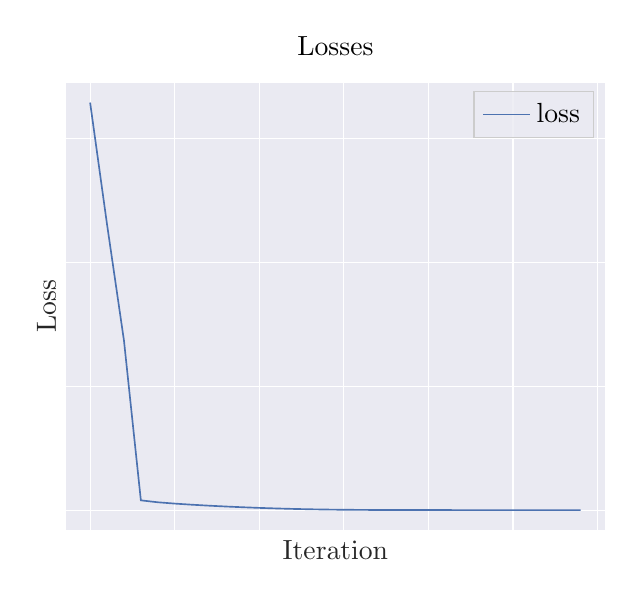
\begin{tikzpicture}
    \definecolor{darkslategray38}{RGB}{38,38,38}
    \definecolor{lavender234234242}{RGB}{234,234,242}
    \definecolor{lightgray204}{RGB}{204,204,204}
    \definecolor{steelblue76114176}{RGB}{76,114,176}
    
    \begin{axis}[
    axis background/.style={fill=lavender234234242},
    axis line style={white},
    legend cell align={left},
    legend style={
      fill opacity=0.8,
      draw opacity=1,
      text opacity=1,
      draw=lightgray204,
      fill=lavender234234242
    },
    tick align=outside,
    title={Losses},
    x grid style={white},
    xlabel=\textcolor{darkslategray38}{Iteration},
    xmajorgrids,
    xmajorticks=false,
    xmin=-1.45, xmax=30.45,
    xtick style={color=darkslategray38},
    y grid style={white},
    ylabel=\textcolor{darkslategray38}{Loss},
    ymajorgrids,
    ymajorticks=false,
    ymin=-0.811937415134162, ymax=17.2548574759625,
    ytick style={color=darkslategray38}
    ]
    \addplot [semithick, steelblue76114176]
    table {%
    0 16.4336395263672
    1 11.5248708724976
    2 6.84751892089844
    3 0.403677195310593
    4 0.325582027435303
    5 0.272632390260696
    6 0.228288665413857
    7 0.189810216426849
    8 0.155834376811981
    9 0.125764444470406
    10 0.0994391441345215
    11 0.0769038200378418
    12 0.0582394674420357
    13 0.0434320122003555
    14 0.0322834849357605
    15 0.0243763793259859
    16 0.0191082842648029
    17 0.0157926622778177
    18 0.013785750605166
    19 0.0125784417614341
    20 0.011825093999505
    21 0.0113176433369517
    22 0.010942131280899
    23 0.0106386914849281
    24 0.0103762578219175
    25 0.0101379100233316
    26 0.00991394650191069
    27 0.00969867128878832
    28 0.00948832742869854
    29 0.00928053446114063
    };
    \addlegendentry{loss}
    \end{axis}
    \end{tikzpicture}    
\end{frame}

\end{document}